\documentclass[conference]{IEEEtran}
\IEEEoverridecommandlockouts
% The preceding line is only needed to identify funding in the first footnote. If that is unneeded, please comment it out.
\usepackage{cite}
\usepackage{amsmath,amssymb,amsfonts}
\usepackage{hyperref}
\usepackage{algorithmic}
\usepackage{graphicx}
\usepackage{textcomp}
\usepackage{xcolor}
\def\BibTeX{{\rm B\kern-.05em{\sc i\kern-.025em b}\kern-.08em
    T\kern-.1667em\lower.7ex\hbox{E}\kern-.125emX}}

\bibliographystyle{IEEEtran}

%% PREAMB : Setting variables
\usepackage{pgfkeys}
\newcommand{\setvalue}[1]{\pgfkeys{/variables/#1}}
\newcommand{\getvalue}[1]{\pgfkeysvalueof{/variables/#1}}
\newcommand{\declare}[1]{%
	\pgfkeys{
		/variables/#1.is family,
		/variables/#1.unknown/.style = {\pgfkeyscurrentpath/\pgfkeyscurrentname/.initial = ##1}
	}%
}
\declare{}
\newcommand{\TITLE}[1]{\setvalue{TITLE= #1}}
\TITLE{Introducting HypoGator: generating coherent hypotheses from biased geo-political data}

\usepackage{braket}
\usepackage{hyperref}
\usepackage{forest}
\usepackage{booktabs}
\usepackage{tikz}

\ifCLASSOPTIONcompsoc
\usepackage[caption=false, font=normalsize, labelfont=sf, textfont=sf]{subfig}
\else
\usepackage[caption=false, font=footnotesize]{subfig}
\fi

\newtheorem{example}{Example}
\newtheorem{definition}{Definition}

\begin{document}

\title{\getvalue{TITLE}\\
%{\footnotesize \textsuperscript{*}Note: Sub-titles are not captured in Xplore and
%should not be used}
%\thanks{Identify applicable funding agency here. If none, delete this.}
}
\author{?}

%\author{\IEEEauthorblockN{1\textsuperscript{st} Given Name Surname}
%\IEEEauthorblockA{\textit{dept. name of organization (of Aff.)} \\
%\textit{name of organization (of Aff.)}\\
%City, Country \\
%email address}
%\and
%\IEEEauthorblockN{2\textsuperscript{nd} Given Name Surname}
%\IEEEauthorblockA{\textit{dept. name of organization (of Aff.)} \\
%\textit{name of organization (of Aff.)}\\
%City, Country \\
%email address}
%\and
%\IEEEauthorblockN{3\textsuperscript{rd} Given Name Surname}
%\IEEEauthorblockA{\textit{dept. name of organization (of Aff.)} \\
%\textit{name of organization (of Aff.)}\\
%City, Country \\
%email address}
%\and
%\IEEEauthorblockN{4\textsuperscript{th} Given Name Surname}
%\IEEEauthorblockA{\textit{dept. name of organization (of Aff.)} \\
%\textit{name of organization (of Aff.)}\\
%City, Country \\
%email address}
%\and
%\IEEEauthorblockN{5\textsuperscript{th} Given Name Surname}
%\IEEEauthorblockA{\textit{dept. name of organization (of Aff.)} \\
%\textit{name of organization (of Aff.)}\\
%City, Country \\
%email address}
%\and
%\IEEEauthorblockN{6\textsuperscript{th} Given Name Surname}
%\IEEEauthorblockA{\textit{dept. name of organization (of Aff.)} \\
%\textit{name of organization (of Aff.)}\\
%City, Country \\
%email address}
%}

\maketitle

\begin{abstract}
[ABSTRACT]
\end{abstract}

\begin{IEEEkeywords}
[Items]
\end{IEEEkeywords}



% !TeX root = 00_paper_main.tex

\section{Introduction}

%%% Part 2: who is the addressee?
Modern \textsc{Knowledge Base Management Systems} allow the ingestion of various data representations, such as relational, graph and full-text data \cite{ibmwatson}. Current KBMS usually ingest reliable data sources, such as encyclopaedic data \cite{ibmwatson}, business data \cite{Saha16} and medical journals and clinical data \cite{WANG201834}. 
%%% Part 1: what I want to say precisely? Which is the broader problem that I want to solve?
Despite such KBMS are able to reconcile different representation towards an uniform one \cite{Niu}, no technique is currently exploited for detecting \textit{contradicting} facts for hypothesis generation: in particular both data collected from on-line social network \cite{Lazer1094} or even medical diagnoses \cite{imihl} may contain contradictions.


\begin{example}
\textit{One of the simplest ways to find contradictions is to check whether there are facts that are both affirmed and denied at the same time. E.g., fact ``Casu Marzu is not a good cheese'' is a rebuttal of the fact ``Casu Marzu is a exquisite cheese''. Alternatively, we can focus on factual representations that do not allow the contemporaneity of two alternative hypotheses, thus violating a functional dependency. E.g., fact ``Yesterday Alice flew to Berlin'' contradicts ``Yesterday Alice took a trip to Kearney'' because Alice cannot be found in two different places at the same time.}
\end{example}

As previously stated, the inherent inconsistency of spurious data sources leads to the generation of conflicting hypotheses in response to a query. The inability of detecting such inconsistencies prohibits to weight how many KBMS facts either support or discard a given hypothesis, thus preventing from correctly ranking the generated hypotheses. This whole scenario demands for a query language which interpretation is able to detect such inconsistencies from the data, and an hypothesis generation task that is able to generate hypotheses which do not contain contradictions. 

%%% Part 4: communicate the Idea that we have (what is an inconsistency)
In order to solve this practical problem, we focus on querying domain-specific knowledge bases containing the aforementioned form of inconsistencies. Such setting allows to use ontologies to represent knowledge, thus allowing to represent both structured (tables), semistructured (wikis, web pages) and unstructured (full texts, videos, images) documents with a uniform representation \cite{DeepDivePhD,Chen14}. MeSH\footnote{\url{https://www.nlm.nih.gov/mesh/}} is an example of an ontology for medical settings. Ontologies prompt the intended semantics and properties of such final representations: they differentiate \textit{entities} from \textit{fillers} (e.g., properties), where the formers are individual units that can be described by different qualities represented as the latter. They also distinguish the \textit{(binary) relationships} involving such entities, and the \textit{facts} providing a description of the observed world, which may involve multiple entities and fillers. Events are a specific case of facts. As previously mentioned, this ideal data description does not prevent the data to be biased: as an example, a different point of view may provide biased factual descriptions, that need to be detected. In order to do so, taxonomies and semantic networks focus more on describing entities and fillers through \textit{relationships}, thus allowing to detect data inconsistencies \cite{Lependu11}.  ICD-11\footnote{\url{https://icd.who.int/}} is a well-known medical taxonomy used to identify and categorize specific diseases and medical procedures uniquely. Ontologies and taxonomies provide the pillars sustaining the HypoGator framework, which consists of a pipeline composed of the following blocks, which are described in more detail in the homonymous paper sections (\S):
	

\begin{itemize}
\item \textbf{Query Interpretation} (\S\ref{sec:querinterp}): any generic query (SPARQL, CYPHER, SQL) is represented as a graph $q$ \cite{Hu0YWZ18} and then used to perform an approximated graph matching with the knowledge base \cite{DeVirgilio2015}.
\item \textbf{Hypothesis Generation} (\S\ref{sec:hypgen}): the previous approximated graph matching generates the preliminar hypotheses $h$: similar or coherent hypotheses are merged (``synthesis''), while conflicting hypotheses are kept separated. %Hypotheses containing inconsistencies are filtered out, while the remaining ones are represented as a graph.
\item \textbf{Hypothesis Evidence and Scoring} (\S\ref{sec:scoring}): before returning such hypotheses, we must know which knowledge base element support the provided hypotheses and which does not. Such evidence extraction is used to provide a first scoring function counting how many supporting facts validate the hypothesis against the remaining ones (either supporting or discarding the hypothesis).
\item \textbf{Hypothesis Query Answering} (\S\ref{sec:synthansw}): after the previous filter phase, each hypothesis $h$ is possibly rewritten into an hypothesis $h'$ maximizing the similarity with $q$. Finally, we rank the hypotheses by combining the previous section's ranking and the edit distance between $h$ and $h'$.
\end{itemize} 


%As a result, this paper provides a formal definition of information inconsistencies, which is later on exploited to define such ranking metric; given a type of facts $t$ associated with a functional dependency $f$, we say that facts $c$ and $\tilde{c}$ of type $t$ are contradictory either if $\tilde{c}$ is the negation of $c$ or the coexistence of $c$ and $\tilde{c}$ in $t$ violates the functional dependency $f$. In order to meet our goal, we represent both events and relationships as multidimensional facts of different types $t$ via common-sense knowledge integration \cite{SpeerCH16}; to each type $t$ we associate a functional dependency by exploiting the ontologies' ability to describe a domain knowledge of interest \cite{FORTINEAU2015573}.

Before providing details of such phases, we analyse the state of the art of query interpretation (\S\ref{sec:queryanswer}), information extraction (\S\ref{sec:rulemining}-\ref{sec:matching}) and knowledge base construction (\S\ref{sec:kbconstr}).

%To improve efficiency and accuracy, we provide some link and rule mining techniques that {\color{red} [TODO]}. To summarize, we make the following contributions:
%\begin{itemize}
%	\item Section description here.
%\end{itemize}
\section{Related Work}
{\color{red} Please note that this section has to be edited accordingly to the type of paper we intend to write.}

\subsection{Natural language query answering}
\begin{itemize}
\item Natural language querying in relational databases: \cite{Li16,Saha16}
\item Natural language querying in graph databases: \cite{Hu0YWZ18}
\end{itemize}

\subsection{Rule Mining}
Miguel, here we should quote the paper on temporal rule mining.

\subsection{Approximated graph pattern matching}
\begin{itemize}
\item Graph matching over dimensions: \cite{PetermannMBPR17}
\item Approximated graph matching: \cite{DeVirgilio2015, ALIGON201520}
\end{itemize}

\subsection{Knowledge Bases}
\begin{itemize}
\item KB with precise information: \cite{ibmwatson}
\item KB with uncertainty: \cite{Chen14, Niu}
\end{itemize}

\begin{table}
	\caption{Association between the variables' instantiation (\textup{\textbf{Candidate}}) to the data associating it (\textup{\textbf{Knowledge Base Facts}}).}
	\begin{tabular}{lp{0.38\textwidth}}
		\toprule
		\textbf{Candidate} & \textbf{Knowledge Base Facts}\\
		\midrule
		Rome & Abigail came back to Rome.\\
		Rome & On September 1988, Abigail moved from Bologna's to La Sapienza University, Rome.\\
		Latium & Yesterday (2018/06/22) Abigail was seen in Latium.\\
		Turin & Abigail was rushed to the ``Umberto I'' hospital in Turin.\\
		Minneapolis & Abigail did a trip to Minneapolis on 1987.\\
		Duluth & Then, Abigail travelled from Minneapolis to Dulduth.\\
		\bottomrule
	\end{tabular}
	\label{tab:datahyp}
\end{table} \begin{figure} 
	\centering
	\subfloat[``\textit{Where did Abigail go?}'']{%
		\label{subfig:q1}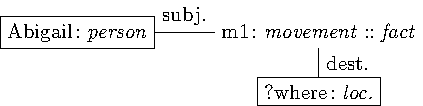
\includegraphics[width=.5\linewidth]{fig/question01.pdf}}
	\hfill
	\subfloat[``\textit{In which places did Calbert not go?}'']{\label{subfig:q4}
		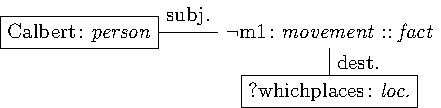
\includegraphics[width=0.45\linewidth]{fig/question04.pdf}}
	\\
	\subfloat[``\textit{Which crimes did Bradford committed before going to jail?}'']{%
		\label{subfig:q2}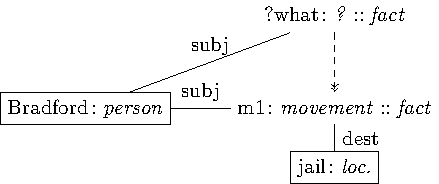
\includegraphics[width=.5\linewidth]{fig/question02.pdf}}
	\hfill
	\subfloat[``\textit{Who robbed the bank before travelling to Paris?}'']{%
		\label{subfig:q2b}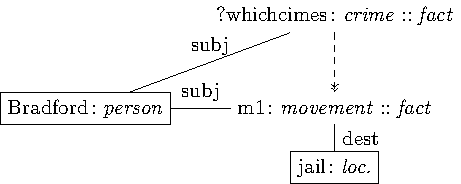
\includegraphics[width=.5\linewidth]{fig/question02bis.pdf}}\\
	\subfloat[``\textit{Which crimes did Bradford committed before going to jail?}'']{%
		\label{subfig:q3}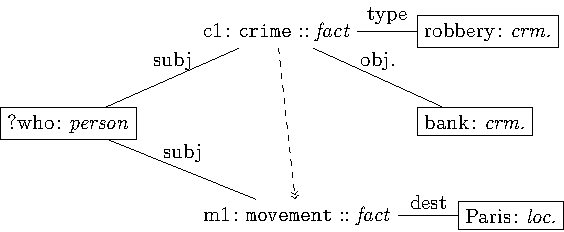
\includegraphics[width=.7\linewidth]{fig/question03.pdf}}\\
	\subfloat[``\textit{Which crime was committed by the person that first travelled to Paris?}'']{%
		\label{subfig:q3b}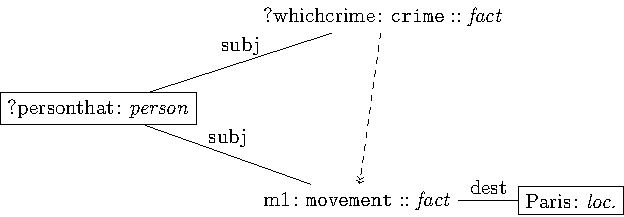
\includegraphics[width=.7\linewidth]{fig/question03b.pdf}}
	\caption{Each entity/filler is represented by a rectangle, facts have no shape and fact's fields are represented by straight edges. Variables are represented by names preceded by a question mark, ?. Temporal associations between facts are represented by dashed edges.}
	\label{fig:querygraph} 
\end{figure}


\section{Query Interpretation}\label{sec:querinterp}
Given that (natural language) queries can be expressed either as a declarative language \cite{Li16,Saha16} or using the same format as the data \cite{Hu0YWZ18,Consens90} (e.g., graphs), this paper uses the latter approach because its representation is language independent. Moreover, the latter approach is also able to express most of the natural language queries of interest within our scenario \texttt{[TODO]}. 

With reference to Figure \ref{fig:querygraph}, each entity and filler can be expressed as a vertex, while each binary relationship can be expressed as a edge, and facts can be expressed as hyperedges connecting different vertices \cite{Fagin83}. Negations can be expressed by juxtaposing the $\neg$ symbol. Natural language uses adverbs or pronouns to identify which are the elements to be returned by the query, namely \textit{variables}, which are represented as nodes (or edges) which name starts with a question mark.  Such variable instantiation can be performed by approximate graph matching the query graph to the data represented in the knowledge base \cite{DeVirgilio2015}, thus creating a set of \textit{morphisms} linking each variable to the corresponding matched KB elements (\textit{candidate}). The KB's subgraph containing all the candidates for a given morphism is an \textit{hypothesis} $h$.  E.g., Table \ref{tab:datahyp} provides in its left column a set of possible hypotheses' candidates generated from the knowledge base data and answering the query ``\textit{Where did Abigail go?}'. 

We now analyse four possible queries of interest within our scenario \texttt{[TODO]}:

\begin{enumerate}
\item \textbf{Return an entity or filler associated to a given fact or relationship.} E.g., for ``\textit{Where did Abigail go?}'' (Figure \ref{subfig:q1}), \textit{go} is the keyword identifying the fact for the specific \texttt{movement} type, while \textit{where} identifies the element to be returned and its type, that is a \textit{location}. Therefore, the query asks for all the facts expressing a movement (\textit{go}) of Abigail towards a specific location (\textit{where}). 
\item \textbf{Return a fact associated to a given fact or relationship.} E.g., in ``\textit{What did Bradford do before going to jail?}'' (Figure \ref{subfig:q2}), the keywords \textit{What} and \textit{do} specify that we need to return a fact which is liked via a temporal association (\textit{before}) to another fact or relationship (\textit{Bradford \dots going to jail}). In this case, the to-be-returned fact may have any possible type. The same question can be also refined to return a specific fact type as in the former example: e.g., ``\textit{Which crimes did Bradford committed before going to jail?}'' (Figure \ref{subfig:q2b}) may specify to return all the facts pertaining to Bradford's criminal record.
\item \textbf{Variables appearing in multiple facts/relationships.} E.g., ``\textit{Who robbed the bank before travelling to Paris?}'' (Figure \ref{subfig:q3}) asks to return an entity (\textit{Who}) which first appears in a \texttt{movement} fact (\textit{Who \dots travelling to Paris}) and, later on, performed a \texttt{crime} (\textit{Who robbed the bank}). We want to return an entity  appearing in two distinct events having a temporal association. This corresponds to a join between two facts where the criminal corresponds to a moving person. 

We can rephrase the same query to return a fact having a variable binding as follows: \textit{Which crime was committed by the person that first travelled to Paris?} (Figure \ref{subfig:q3b}). In this case the variable binding is made explicit by the keywords \textit{person} and \textit{that}, while \textit{Which} remarks that we now want to return only the criminal facts.
\item \textbf{Negated queries.} E.g., for ``\textit{In which places did Calbert not go?}'' (Figure \ref{subfig:q4}), we can provide either all the \textit{places} appearing in negated place relationships or \texttt{movement} facts, or return a set of all the possible \textit{places} not appearing in non-negated \texttt{place} relationships and \texttt{movement} facts.  Please note that such queries can be directly expressed in graph query languages which, on the other hand, do not usually query data that may contain negations. On the other hand, current graph pattern matching frameworks may only express positive facts.
\end{enumerate}


\section{Hypothesis Generation}\label{sec:hypgen}
The hypotheses generator acts as the first part for the query evaluation, which identifies and aggregates the data in the Knowledge Base (approximately) matching the query.

Let us now focus on hypotheses containing only one candidate as in Table \ref{tab:datahyp}; by using some geographical taxonomy as the one in Figure \ref{tree:geotree}, we may also coarsen the former candidates in order to get a better hypothesis' support: we have that the hypothesis with candidate (h.w.c.) \textit{Italy} is supported by three entities over five, while h.w.c. \textit{USA} or \textit{Minnesota} is supported by two entities over five. Please note that trivial hypotheses  should be discarded: an hypothesis is trivial when it contains all the other generated hypotheses (e.g., ``\textit{World}''). Please note that single candidates cannot be inconsistent with themselves, because conflicting candidates are separated in different hypotheses by definition (e.g., all the cities are different to each other, except from Rome that appears twice). Nevertheless, not all the hypotheses are inconsistent to each other (e.g., ``\textit{Rome}'' is compatible with ``\textit{Latium}'' and ``\textit{Italy}'', but not with ``\textit{Turin}'' and ``\textit{Piedmont}'').

\begin{figure}
\centering
\begin{forest}
	for tree={fit=band}
	[\textit{location} [World
	[Italy
	[Latium [Rome]]
	[Piedmont [Turin]]
	]
	[USA
	[Minnesota
	[Minneapolis]
	[Duluth]
	]
	]
	]
	]
\end{forest}
\caption{An example of a geographical taxonomy for geographical dimensions (\textit{location}). Taxonomies may be used to aggregate compatible hypotheses.}\label{tree:geotree}
\end{figure}

Last, this approach can be generalized over multiple candidates by combining multiple hierarchies together as described in \cite{PetermannMBPR17}, where candidates may be extracted at different possible representation levels \texttt{[Is this enough or do I have to provide more details on how I would do that?]}.
\section{Hypothesis Evidence and Scoring}\label{sec:scoring}
In contrast to the evidence in the former section, having coherent candidates does not prevent us from having hypotheses that either contain contradictions or are contradicted by other facts or relationships. It is then required to associate each generated hypothesis with the set of facts and relationships providing either evidence or counterevidence. 

Let us analyse some possible inconsistencies: if we suppose that the relationship ``\textit{Abigail has never been in the USA}'' is stored within our knowledge base, then we now that this evidence contradicts the facts in Table \ref{tab:datahyp} generating the candidates ``\textit{Minneapolis}'' and ``\textit{Duluth}''. On the other hand, the relationship ``\textit{Abigail was born in Detroit on 1989}''  contradicts with the second ``\textit{Rome}'' candidate, because the entity \textit{Abigail} did not existed prior to 1989. Last, the fact ``\textit{On the 22\textsuperscript{nd} of June 2018, Abigail died in Turin}'' contradicts with the hypothesis ``\textit{Latium}'' because the same person cannot be located in two different places at the same time. 

The former inconsistencies may be observed by comparing different KB facts and relationships with the hypothesis, which combination describes a subset of the whole knowledge graph, $\kappa$. We can now represent facts and tuples from $\kappa$ as tuples, thus allowing to use logical inconsistent detection frameworks which are independent from the graph representation of the data \cite{MINOUX19881}. Rules may be directly provided by the ontologies' TBox-es \texttt{[cite:TODO]}, which describe the correlations between different facts and relationships and provide an homogeneous representation of different facts and relationships. E.g., the TBox may state that each \texttt{movement} fact towards a given destination at a given time implies a \texttt{location} relationship of the same subject at the same time. After converting each possible fact and relationships into ``finer-grained'' facts and relationships, it is now possible to recognize all the spatio-temporal inconsistencies as in \cite{gmmp18}. This approach can  be therefore extended to any other type of inconsistencies foreseen by the  TBox rules in ontologies. 

Last, we can now measure its discrepancies via support scores, thus providing a first ranking of the generated hypotheses. 
\section{Hypothesis  Query Answering}\label{sec:synthansw}
As previously stated, each ``minimal'' connected (hyper)graph containing the candidates describes an hypothesis $h$. Now, we want to align $h$ towards the query representation: such alignment can be represented by instantiating the query variables in $q$ with the candidates, thus obtaining the to-be-returned hypothesis $h'$. Given that $h$ was obtained through approximate graph matching of $q$, we know that the greater the edit distance between the two $h$ and $h'$, the less the reliability on $h'$ as a possible candidate. By doing so we assign higher scores to the hypotheses that are directly represented within the data, and inferior ones to all the remaining hypotheses that were generated over imprecise(?) inference rules. The combination of the support measure with the edit distance provides the score assigned to $h'$.
%\section{Preliminaries}
\begin{definition}[Knowledge Base]
A \textbf{knowledge base} $KB$ is a graph containing ground atoms.
\end{definition}
\medskip

\begin{definition}[Query]
A \textbf{query} $q$ is a graph containing unbounded variables $?x$ to which a common-sense type $\tau$ is associated. $U_q$ is a finite set of all the unbounded atoms in $q$.
\end{definition}
\medskip

\begin{definition}[Answer]
An \textbf{answer} $A$ to a query $q$ over a knowledge base $KB$ (namely, $q(KB)=A$) is a set of distinct finite functions $\alpha:U_q\to KB$, named \textbf{candidate alternative}.

We denote $\alpha\oplus q$ as the operation replacing each unbounded atom $?x$ in the query $q$ with the candidate $\alpha(?x)$.
\end{definition}
\medskip

\begin{definition}[Hypothesis]
An \textbf{hypothesis} $h$ supporting a candidate alternative $\alpha$ for query $q$ is a subgraph of $KB$ matching with $q$ ($ h\subseteq KB\wedge \textup{sim}(h,\alpha\oplus q)$).
\end{definition}
\medskip

\begin{definition}[Support]
For each hypothesis $h$ generated from a knowledge base $KB$, the support is a pair $s(h)=\braket{C,\tilde{C}}$, where $C$ is a set of ground $KB$ atoms validating $h$ and $\tilde{C}$ is a set of facts discarding the hypothesis.
\end{definition}

As a consequence of the support definition, we want enforce that the hypotheses scoring function $\sigma$ must enjoy the following properties:
\begin{itemize}
\item if $s(h)=\braket{C,\emptyset}$ with $C\neq \emptyset$, then $h$ is ``global truth'' in $KB$ and then $\sigma(h)=1$.
\item if $s(h)=\braket{\emptyset, \tilde{C}}$ with $C\neq \emptyset$, then $h$ is ``global falsehood'' in $KB$ and then $\sigma(h)=0$.
\item $0<\sigma(h)<1$ otherwise.
\end{itemize}
\medskip

{\color{red}[More definitions compliant with the learning steps]} In the learning phase, we can approximate each query $q$ with a set of probable hypotheses that may be returned by the $KB$

Less equal ($<=$) is $\leq$: \url{http://web.ift.uib.no/Teori/KURS/WRK/TeX/symALL.html}  %% preliminaries = optional causes
%\section{Architecture}
{\color{red} Fragment 1:} Our architecture is based upon the Closed World Assumption: each hypothesis that cannot be directly generated or inferred by our internal data representation should be considered inadmissible. 

{\color{red} Fragment 2:} The system architecture which is used to query the data is defined by the following steps:
\begin{enumerate}
	\item Given a knowledge base $KB$, perform the query $q$ returning an answer $A=\Set{\alpha_1,\dots,\alpha_n}$
	\item For each candidate alternative $\alpha_i$, return a set of hypotheses $\Set{h^1_i,\dots h^m_i}$
	\item For each hypothesis $h^j_i$, evaluate its support $s(h^j_i)$ and rank it through $\sigma$.
\end{enumerate}


%\section{Algorithm}
\begin{itemize}
\item Rename this section with the algorithm name.
\item Are there more than just one algorithm to describe?
\item Shall we describe the main pipeline instead, and use other papers as back references?
\end{itemize}
%\section{Experimental Evaluation}

{\color{red} Fragment 3:} In order to evaluate our architecture, we use the LDC dataset {\color{red}[TODO: which?]}, in which each query $q$ is described as a set of hypotheses with its support set. Therefore, {\color{red} we must define a similarity score between support sets for each hypothesis in order to evaluate the compliance of our KB with respect to the returned hypotheses.}
\section{Conclusion}
\section*{Acknowledgment}

\texttt{[DARPA Project ?]}
%The preferred spelling of the word ``acknowledgment'' in America is without 
%an ``e'' after the ``g''. Avoid the stilted expression ``one of us (R. B. 
%G.) thanks $\ldots$''. Instead, try ``R. B. G. thanks$\ldots$''. Put sponsor 
%acknowledgments in the unnumbered footnote on the first page.
\bibliography{bibliography}

%
%\subsection{Maintaining the Integrity of the Specifications}
%
%The IEEEtran class file is used to format your paper and style the text. All margins, 
%column widths, line spaces, and text fonts are prescribed; please do not 
%alter them. You may note peculiarities. For example, the head margin
%measures proportionately more than is customary. This measurement 
%and others are deliberate, using specifications that anticipate your paper 
%as one part of the entire proceedings, and not as an independent document. 
%Please do not revise any of the current designations.
%
%\section{Prepare Your Paper Before Styling}
%Before you begin to format your paper, first write and save the content as a 
%separate text file. Complete all content and organizational editing before 
%formatting. Please note sections \ref{AA}--\ref{SCM} below for more information on 
%proofreading, spelling and grammar.
%
%Keep your text and graphic files separate until after the text has been 
%formatted and styled. Do not number text heads---{\LaTeX} will do that 
%for you.
%
%\subsection{Abbreviations and Acronyms}\label{AA}
%Define abbreviations and acronyms the first time they are used in the text, 
%even after they have been defined in the abstract. Abbreviations such as 
%IEEE, SI, MKS, CGS, ac, dc, and rms do not have to be defined. Do not use 
%abbreviations in the title or heads unless they are unavoidable.
%
%\subsection{Units}
%\begin{itemize}
%\item Use either SI (MKS) or CGS as primary units. (SI units are encouraged.) English units may be used as secondary units (in parentheses). An exception would be the use of English units as identifiers in trade, such as ``3.5-inch disk drive''.
%\item Avoid combining SI and CGS units, such as current in amperes and magnetic field in oersteds. This often leads to confusion because equations do not balance dimensionally. If you must use mixed units, clearly state the units for each quantity that you use in an equation.
%\item Do not mix complete spellings and abbreviations of units: ``Wb/m\textsuperscript{2}'' or ``webers per square meter'', not ``webers/m\textsuperscript{2}''. Spell out units when they appear in text: ``. . . a few henries'', not ``. . . a few H''.
%\item Use a zero before decimal points: ``0.25'', not ``.25''. Use ``cm\textsuperscript{3}'', not ``cc''.)
%\end{itemize}
%
%\subsection{Equations}
%Number equations consecutively. To make your 
%equations more compact, you may use the solidus (~/~), the exp function, or 
%appropriate exponents. Italicize Roman symbols for quantities and variables, 
%but not Greek symbols. Use a long dash rather than a hyphen for a minus 
%sign. Punctuate equations with commas or periods when they are part of a 
%sentence, as in:
%\begin{equation}
%a+b=\gamma\label{eq}
%\end{equation}
%
%Be sure that the 
%symbols in your equation have been defined before or immediately following 
%the equation. Use ``\eqref{eq}'', not ``Eq.~\eqref{eq}'' or ``equation \eqref{eq}'', except at 
%the beginning of a sentence: ``Equation \eqref{eq} is . . .''
%
%\subsection{\LaTeX-Specific Advice}
%
%Please use ``soft'' (e.g., \verb|\eqref{Eq}|) cross references instead
%of ``hard'' references (e.g., \verb|(1)|). That will make it possible
%to combine sections, add equations, or change the order of figures or
%citations without having to go through the file line by line.
%
%Please don't use the \verb|{eqnarray}| equation environment. Use
%\verb|{align}| or \verb|{IEEEeqnarray}| instead. The \verb|{eqnarray}|
%environment leaves unsightly spaces around relation symbols.
%
%Please note that the \verb|{subequations}| environment in {\LaTeX}
%will increment the main equation counter even when there are no
%equation numbers displayed. If you forget that, you might write an
%article in which the equation numbers skip from (17) to (20), causing
%the copy editors to wonder if you've discovered a new method of
%counting.
%
%{\BibTeX} does not work by magic. It doesn't get the bibliographic
%data from thin air but from .bib files. If you use {\BibTeX} to produce a
%bibliography you must send the .bib files. 
%
%{\LaTeX} can't read your mind. If you assign the same label to a
%subsubsection and a table, you might find that Table I has been cross
%referenced as Table IV-B3. 
%
%{\LaTeX} does not have precognitive abilities. If you put a
%\verb|\label| command before the command that updates the counter it's
%supposed to be using, the label will pick up the last counter to be
%cross referenced instead. In particular, a \verb|\label| command
%should not go before the caption of a figure or a table.
%
%Do not use \verb|\nonumber| inside the \verb|{array}| environment. It
%will not stop equation numbers inside \verb|{array}| (there won't be
%any anyway) and it might stop a wanted equation number in the
%surrounding equation.
%
%\subsection{Some Common Mistakes}\label{SCM}
%\begin{itemize}
%\item The word ``data'' is plural, not singular.
%\item The subscript for the permeability of vacuum $\mu_{0}$, and other common scientific constants, is zero with subscript formatting, not a lowercase letter ``o''.
%\item In American English, commas, semicolons, periods, question and exclamation marks are located within quotation marks only when a complete thought or name is cited, such as a title or full quotation. When quotation marks are used, instead of a bold or italic typeface, to highlight a word or phrase, punctuation should appear outside of the quotation marks. A parenthetical phrase or statement at the end of a sentence is punctuated outside of the closing parenthesis (like this). (A parenthetical sentence is punctuated within the parentheses.)
%\item A graph within a graph is an ``inset'', not an ``insert''. The word alternatively is preferred to the word ``alternately'' (unless you really mean something that alternates).
%\item Do not use the word ``essentially'' to mean ``approximately'' or ``effectively''.
%\item In your paper title, if the words ``that uses'' can accurately replace the word ``using'', capitalize the ``u''; if not, keep using lower-cased.
%\item Be aware of the different meanings of the homophones ``affect'' and ``effect'', ``complement'' and ``compliment'', ``discreet'' and ``discrete'', ``principal'' and ``principle''.
%\item Do not confuse ``imply'' and ``infer''.
%\item The prefix ``non'' is not a word; it should be joined to the word it modifies, usually without a hyphen.
%\item There is no period after the ``et'' in the Latin abbreviation ``et al.''.
%\item The abbreviation ``i.e.'' means ``that is'', and the abbreviation ``e.g.'' means ``for example''.
%\end{itemize}
%An excellent style manual for science writers is \cite{b7}.
%
%\subsection{Authors and Affiliations}
%\textbf{The class file is designed for, but not limited to, six authors.} A 
%minimum of one author is required for all conference articles. Author names 
%should be listed starting from left to right and then moving down to the 
%next line. This is the author sequence that will be used in future citations 
%and by indexing services. Names should not be listed in columns nor group by 
%affiliation. Please keep your affiliations as succinct as possible (for 
%example, do not differentiate among departments of the same organization).
%
%\subsection{Identify the Headings}
%Headings, or heads, are organizational devices that guide the reader through 
%your paper. There are two types: component heads and text heads.
%
%Component heads identify the different components of your paper and are not 
%topically subordinate to each other. Examples include Acknowledgments and 
%References and, for these, the correct style to use is ``Heading 5''. Use 
%``figure caption'' for your Figure captions, and ``table head'' for your 
%table title. Run-in heads, such as ``Abstract'', will require you to apply a 
%style (in this case, italic) in addition to the style provided by the drop 
%down menu to differentiate the head from the text.
%
%Text heads organize the topics on a relational, hierarchical basis. For 
%example, the paper title is the primary text head because all subsequent 
%material relates and elaborates on this one topic. If there are two or more 
%sub-topics, the next level head (uppercase Roman numerals) should be used 
%and, conversely, if there are not at least two sub-topics, then no subheads 
%should be introduced.
%
%\subsection{Figures and Tables}
%\paragraph{Positioning Figures and Tables} Place figures and tables at the top and 
%bottom of columns. Avoid placing them in the middle of columns. Large 
%figures and tables may span across both columns. Figure captions should be 
%below the figures; table heads should appear above the tables. Insert 
%figures and tables after they are cited in the text. Use the abbreviation 
%``Fig.~\ref{fig}'', even at the beginning of a sentence.
%
%\begin{table}[htbp]
%\caption{Table Type Styles}
%\begin{center}
%\begin{tabular}{|c|c|c|c|}
%\hline
%\textbf{Table}&\multicolumn{3}{|c|}{\textbf{Table Column Head}} \\
%\cline{2-4} 
%\textbf{Head} & \textbf{\textit{Table column subhead}}& \textbf{\textit{Subhead}}& \textbf{\textit{Subhead}} \\
%\hline
%copy& More table copy$^{\mathrm{a}}$& &  \\
%\hline
%\multicolumn{4}{l}{$^{\mathrm{a}}$Sample of a Table footnote.}
%\end{tabular}
%\label{tab1}
%\end{center}
%\end{table}
%
%\begin{figure}[htbp]
%%\centerline{\includegraphics{fig1.png}}
%\caption{Example of a figure caption.}
%\label{fig}
%\end{figure}
%
%Figure Labels: Use 8 point Times New Roman for Figure labels. Use words 
%rather than symbols or abbreviations when writing Figure axis labels to 
%avoid confusing the reader. As an example, write the quantity 
%``Magnetization'', or ``Magnetization, M'', not just ``M''. If including 
%units in the label, present them within parentheses. Do not label axes only 
%with units. In the example, write ``Magnetization (A/m)'' or ``Magnetization 
%\{A[m(1)]\}'', not just ``A/m''. Do not label axes with a ratio of 
%quantities and units. For example, write ``Temperature (K)'', not 
%``Temperature/K''.







%Please number citations consecutively within brackets \cite{b1}. The 
%sentence punctuation follows the bracket \cite{b2}. Refer simply to the reference 
%number, as in \cite{b3}---do not use ``Ref. \cite{b3}'' or ``reference \cite{b3}'' except at 
%the beginning of a sentence: ``Reference \cite{b3} was the first $\ldots$''
%
%Number footnotes separately in superscripts. Place the actual footnote at 
%the bottom of the column in which it was cited. Do not put footnotes in the 
%abstract or reference list. Use letters for table footnotes.
%
%Unless there are six authors or more give all authors' names; do not use 
%``et al.''. Papers that have not been published, even if they have been 
%submitted for publication, should be cited as ``unpublished'' \cite{b4}. Papers 
%that have been accepted for publication should be cited as ``in press'' \cite{b5}. 
%Capitalize only the first word in a paper title, except for proper nouns and 
%element symbols.
%
%For papers published in translation journals, please give the English 
%citation first, followed by the original foreign-language citation \cite{b6}.

%\begin{thebibliography}{00}
%\bibitem{b1} G. Eason, B. Noble, and I. N. Sneddon, ``On certain integrals of Lipschitz-Hankel type involving products of Bessel functions,'' Phil. Trans. Roy. Soc. London, vol. A247, pp. 529--551, April 1955.
%\bibitem{b2} J. Clerk Maxwell, A Treatise on Electricity and Magnetism, 3rd ed., vol. 2. Oxford: Clarendon, 1892, pp.68--73.
%\bibitem{b3} I. S. Jacobs and C. P. Bean, ``Fine particles, thin films and exchange anisotropy,'' in Magnetism, vol. III, G. T. Rado and H. Suhl, Eds. New York: Academic, 1963, pp. 271--350.
%\bibitem{b4} K. Elissa, ``Title of paper if known,'' unpublished.
%\bibitem{b5} R. Nicole, ``Title of paper with only first word capitalized,'' J. Name Stand. Abbrev., in press.
%\bibitem{b6} Y. Yorozu, M. Hirano, K. Oka, and Y. Tagawa, ``Electron spectroscopy studies on magneto-optical media and plastic substrate interface,'' IEEE Transl. J. Magn. Japan, vol. 2, pp. 740--741, August 1987 [Digests 9th Annual Conf. Magnetics Japan, p. 301, 1982].
%\bibitem{b7} M. Young, The Technical Writer's Handbook. Mill Valley, CA: University Science, 1989.
%\end{thebibliography}
%\vspace{12pt}
%\color{red}
%IEEE conference templates contain guidance text for composing and formatting conference papers. Please ensure that all template text is removed from your conference paper prior to submission to the conference. Failure to remove the template text from your paper may result in your paper not being published.

\end{document}